\documentclass[tikz,border=3pt]{standalone}
\usepackage[utf8]{inputenc}
\usepackage[T1]{fontenc}
\usepackage{lmodern}
\renewcommand{\familydefault}{\sfdefault}
\usepackage{sansmath}\sansmath
\usepackage{chemfig}
\usepackage{pgfplots}\pgfplotsset{compat=1.18,/pgf/number format/use comma,/pgf/number format/1000 sep={.}}
\usetikzlibrary{arrows.meta,calc,positioning,decorations.pathmorphing,patterns}
% paleta del sitio
\definecolor{nar}{HTML}{E8680C}\definecolor{narc}{HTML}{FFB35C}\definecolor{hielo}{HTML}{FFF3E8}
\definecolor{tinta}{HTML}{1D1D1F}\definecolor{gris}{HTML}{6E6E73}\definecolor{lila}{HTML}{7C5CF0}
\definecolor{azul}{HTML}{2F6FD6}\definecolor{menta}{HTML}{17A673}\definecolor{coral}{HTML}{E8342A}
\begin{document}
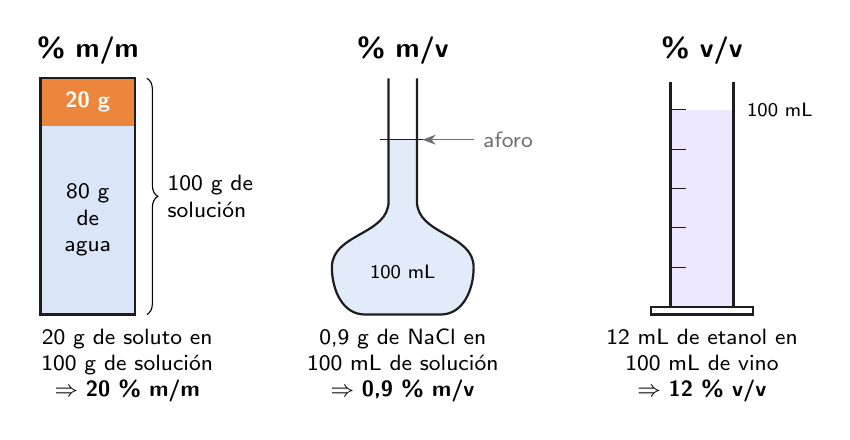
\begin{tikzpicture}[font=\small]
% --- % m/m: barra de 100 g de solucion
\node[font=\bfseries] at (0.6,3.35) {\% m/m};
\fill[azul!18] (0,0) rectangle (1.2,2.4);
\fill[nar!80] (0,2.4) rectangle (1.2,3.0);
\draw[tinta,thick] (0,0) rectangle (1.2,3.0);
\node[white,font=\footnotesize\bfseries] at (0.6,2.7) {20 g};
\node[font=\footnotesize,align=center] at (0.6,1.2) {80 g\\de\\agua};
\draw[decorate,decoration={brace,amplitude=4pt}] (1.35,3.0) -- (1.35,0) node[midway,right=4pt,font=\footnotesize,align=left] {100 g de\\solución};
\node[align=center,font=\footnotesize] at (1.1,-0.65) {20 g de soluto en\\100 g de solución\\$\Rightarrow$ \textbf{20 \% m/m}};
% --- % m/v: matraz aforado de 100 mL
\begin{scope}[shift={(4.6,0)},scale=1.2]
\path[fill=azul!14] (-0.15,1.85) -- (-0.15,1.2) to[out=-90,in=90] (-0.75,0.5) to[out=-90,in=180] (-0.4,0) -- (0.4,0)
   to[out=0,in=-90] (0.75,0.5) to[out=90,in=-90] (0.15,1.2) -- (0.15,1.85) -- cycle;
\draw[tinta,thick] (-0.15,2.5) -- (-0.15,1.2) to[out=-90,in=90] (-0.75,0.5) to[out=-90,in=180] (-0.4,0) -- (0.4,0)
   to[out=0,in=-90] (0.75,0.5) to[out=90,in=-90] (0.15,1.2) -- (0.15,2.5);
\draw[tinta] (-0.24,1.85) -- (0.24,1.85);
\node[font=\scriptsize] at (0,0.45) {100 mL};
\end{scope}
\node[font=\bfseries] at (4.6,3.35) {\% m/v};
\draw[gris,-{Stealth}] (5.5,2.22) -- (4.85,2.22) node[pos=0,right,font=\footnotesize] {aforo};
\node[align=center,font=\footnotesize] at (4.6,-0.65) {0,9 g de NaCl en\\100 mL de solución\\$\Rightarrow$ \textbf{0,9 \% m/v}};
% --- % v/v: probeta de 100 mL
\begin{scope}[shift={(8.4,0)}]
\fill[lila!14] (-0.4,0.1) rectangle (0.4,2.6);
\draw[tinta,thick] (-0.4,2.95) -- (-0.4,0.1) -- (0.4,0.1) -- (0.4,2.95);
\draw[tinta,thick] (-0.65,0) rectangle (0.65,0.1);
\foreach \y in {0.6,1.1,1.6,2.1,2.6} \draw[tinta] (-0.4,\y) -- (-0.2,\y);
\node[font=\scriptsize,anchor=west] at (0.45,2.6) {100 mL};
\end{scope}
\node[font=\bfseries] at (8.4,3.35) {\% v/v};
\node[align=center,font=\footnotesize] at (8.4,-0.65) {12 mL de etanol en\\100 mL de vino\\$\Rightarrow$ \textbf{12 \% v/v}};
\end{tikzpicture}
\end{document}
